% !TEX root = perelman-geometry.tex
%!TEX TS-program = pdflatex
%!TEX encoding = UTF-8 Unicode

\setchapterpreamble[o]{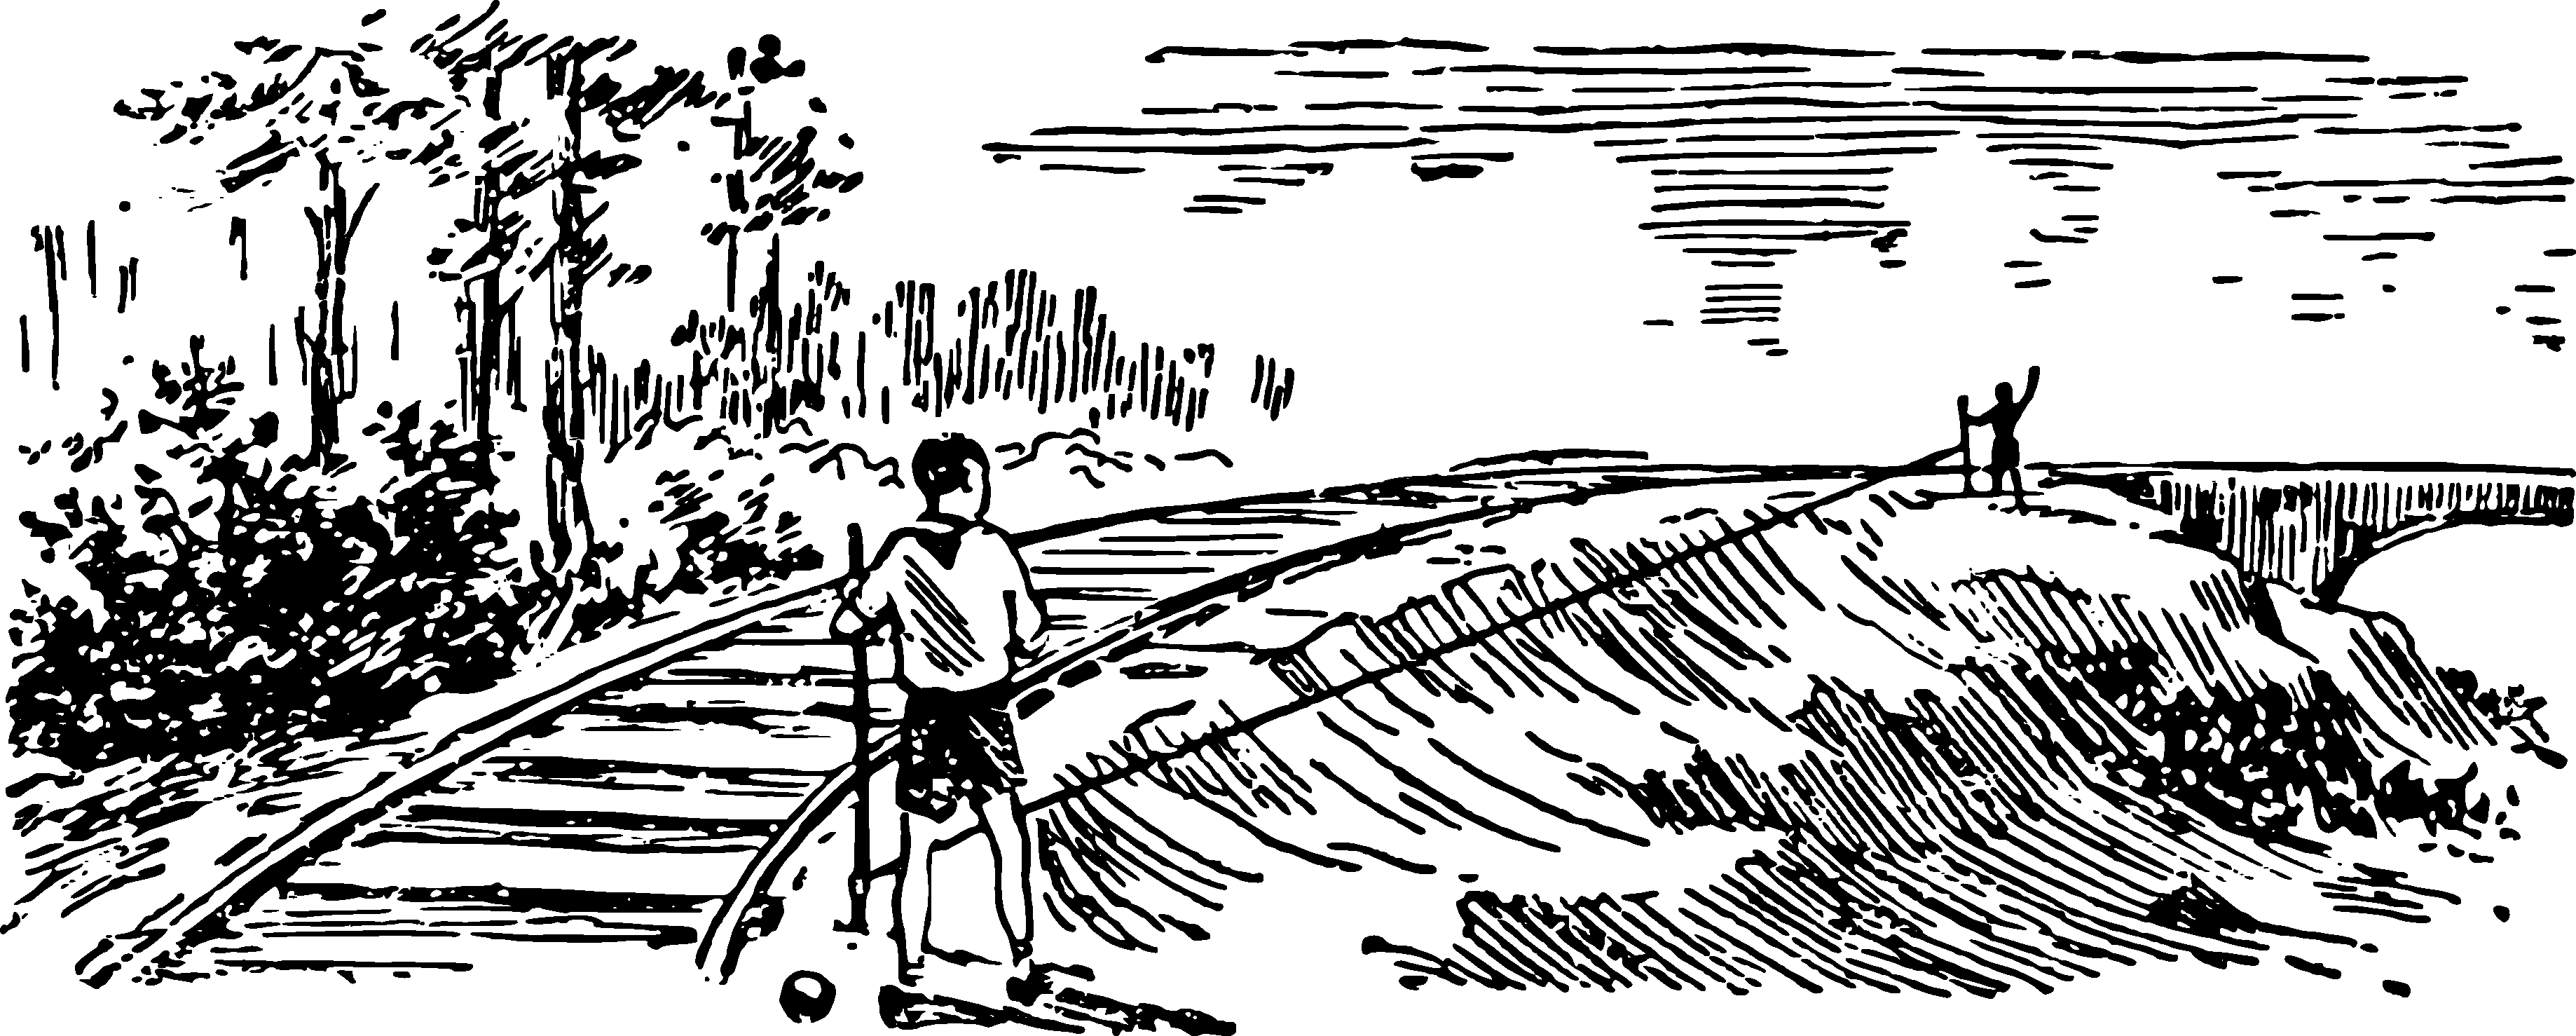
\includegraphics[width=1.2\textwidth]{figures/ch-04/fig-ch-04-head.pdf}\bigskip}

\chapter{Geometry on the Road}
\label{ch-04}

\section{The art of measuring by steps}
\label{sec-4.1}


While out for a countryside walk along a railway track or on a highway, you can perform a series of interesting geometric exercises.

First, use the highway to measure the length of your step and walking speed. This will allow you to -- measure distances by steps -- an art that is acquired quite easily after a short practise. The main thing here is to get used to making steps of the same length every time, i.e., to adopt a certain `measured' gait.

On the highway, every 100 meters, there is a white stone; by walking such a 100-meter interval with your usual `measured' step and counting the number of steps, you can easily find the average length of your step. Such measurement should be repeated annually, for example, every spring, because the length of a step, especially in young people, does not remain constant.

It is worth noting an interesting relationship discovered by repeated measurements: the average length of an adult's step is approximately half of their height, measured to eye level. For example, if a person's height to their eyes is 1 meter 40 centimetres, then the length of their step is about 70 centimetres. It's interesting to verify this rule whenever possible.

\begin{center}
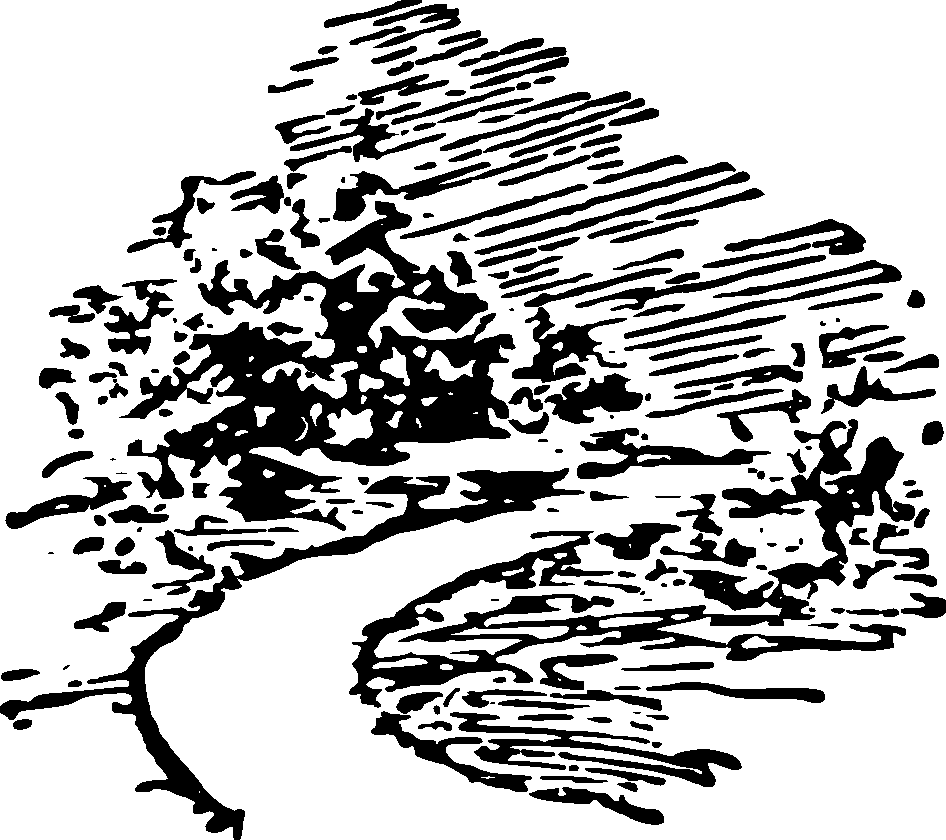
\includegraphics[width=0.3\textwidth]{figures/ch-04/fig-ch-04-tail.pdf}
\end{center}


















